% Document template based on LNCS, adapted by Matt Welsh <mdw@cs.berkeley.edu> and Mark Hempstead<mhempstead@coe.drexel.edu>

\documentclass{article}
\usepackage{program}
\usepackage{acm-style10} % ACM proceedings formatting
\usepackage{times}       % Use Adobe Times font set
\usepackage{epsfig,twocolumn}
\usepackage{lipsum}
\usepackage{url}
\usepackage[english]{babel} % mdw: Required to get good hyphenation on RH6.0
                            % (fixed in RH6.1)
\usepackage{graphicx}
\graphicspath{{figures/}}
\usepackage{color}
\usepackage{soul}
\usepackage[font=small,labelfont=bf]{caption}
\usepackage{appendix}
\usepackage{lscape}

% Source code listing setup
\usepackage{listings}
\lstset{language=C}
\lstset{
	language=C,
    frame=L,
    captionpos=b,
    tabsize=2,
    basicstyle=\ttfamily\scriptsize,
    breaklines=true,
    showstringspaces=false,
}


% DO NOT EDIT THE BELOW BLOCK OF CODE
\def\dsp{\def\baselinestretch{1.10}}
\dsp
\newcommand{\XXXnote}[1]{{\bf\color{red} XXX: #1}}
\setlength{\textheight}{9.25in}
\setlength{\columnsep}{0.33in}
\setlength{\textwidth}{7.4in}
\setlength{\footskip}{0.0in}
\setlength{\topmargin}{-0.25in}
\setlength{\headheight}{0.0in}
\setlength{\headsep}{0.0in}
\setlength{\oddsidemargin}{-.45in}
\setlength{\parindent}{1pc}
\pagestyle{empty}
\begin{document}
\date{\aufnt May 13, 2016}

%%%%%%%%%%%% THIS IS WHERE WE PUT IN THE TITLE AND AUTHORS %%%%%%%%%%%%

% Title here
\title{\ttlfnt Designing Architecture for Multi-Accelerator Applications}

% Author names, affiliations, and e-mail below
\author{{\aufnt Riley Wood} \\ 
{\affaddr Computer Architecture Lab} \\
{\affaddr Tufts University} \\ 
{\affaddr rjw245@gmail.com}}

\maketitle
%\copyrightspace
\thispagestyle{empty}

%%%%%%%%%%%%%  ABSTRACT GOES HERE %%%%%%%%%%%%%%

\begin{abstract}
This paper summarizes my research on hardware accelerators and details the work I have done regarding the development of an architecture to support multi-accelerator applications. Computer architects are preparing to confront an impending limit on the number of transistors on chip that can be used at any given time. This utilization wall will limit the extent to which computers can benefit from increasing transistor counts. Specializing the transistors on chip is one solution which seems to be gaining traction among the research community and in industry. As researchers pursue this option, they have begun to develop new accelerator-rich architectures (ARAs) to handle the challenges posed by specialization. For researchers to conclusively evaluate and compare these architectures, they will need a catalog of applications which use many accelerators. This work focuses on the design of an architecture upon which such applications can be built. The architecture is developed for the Zynq-7000 line of systems-on-chip and serves as a baseline architecture for ARA research. This work was conducted during the spring of 2016 under the supervision of Professor Mark Hempstead as part of an independent study in hardware accelerators.
\end{abstract}

%%%%%%%%%%%%%  BODY OF PAPER GOES HERE %%%%%%%%%%%%%%

\section{Introduction}

\paragraph{The Motivation for Specialization}
It used to be that as transistors grew smaller, chip power consumption would remain constant due to a principle known as Dennard scaling~\cite{dennardscaling}. Since 2006, Dennard scaling has begun to fail due to the fact that sub-micron sized transistors are more susceptible to leakage current and other non-ideal phenomena~\cite{dennard_end}. This means that placing more transistors on chip incurs greater power consumption, yet modern computers are unable to consume any more power and still be kept cool. For example, the power consumption of Intel CPUs plateaued back in 2006~\cite{hruska_2012}. To continue increasing the number of transistors on chip and stay within power budget, designers will have to selectively under-clock or turn off portions of the chip. As the number of transistors on chip grows, a smaller and smaller percentage of them will be usable at any given time. This \textit{utilization wall}, as it is called by Venkatesh et al.~\cite{Venkatesh:2010}, threatens to limit the extent to which computers can benefit from increasing transistor counts in the future.

Several solutions to the utilization wall have been proposed, including shrinking the number of transistors on chip, ``dimming'' regions of the chip, developing new, more efficient transistor technologies, and specializing groups of transistors. The first of these, shrinking transistor counts, clearly means the end of Moore's Law scaling. This has been called the ``most pessimistic'' solution to the problem~\cite{Taylor:2012}, and understandably, many in industry are hesitant to make such a big concession. ``Dimming'' technologies make the transistors on chip more energy-efficient, thereby increasing the number of transistors that can be used while staying within power budgets. However, these techniques often cause a decrease in performance. Dynamic voltage and frequency scaling (DVFS) is a common technique to reduce the power consumption of transistors when high performance is not required. Some work has been done to make DVFS even more effective for modern architectures~\cite{better_dvfs}. Other work targets energy efficiency by trying to make transistors more reusable. For example, DySER from the University of Wisconsin-Madison is an element of the processor pipeline that can be reconfigured to implement one of multiple functions~\cite{dyser}. Because DySER is reconfigurable, energy is only expended on the data path that is currently configured. This saves energy compared to architectures where idle data paths still consume power. The third approach---the development of new transistor tech---addresses the failure of Dennard scaling by abandoning CMOS altogether. Some of the work in this field includes tunnel field-effect transistors (TFETs)~\cite{tfets} which use quantum tunneling to implement a switch, and nano electro-mechanical switches (NEMS)~\cite{nems} which take advantage of the power efficiency of nano-switch technology. Lastly, specialization addresses power limitations by spreading computation across an array of specialized blocks of transistors, called accelerators. Rather than have a monolithic processor do the majority of computation and offload a small portion to specialized hardware (as is the norm today), the vision for specialization in the future has computation bouncing between many specialized regions of the chip~\cite{Taylor:2012}. Because there are more transistors on chip than can be used at any one time, area can be ``spent'' on accelerators specialized for certain computations. These accelerators use fewer transistors than a general-purpose processor to implement specific functionality. Thus, on a fully specialized system, the computer will use a minimal number of transistors at any given time, thereby maintaining performance gains despite the utilization wall.

Accelerators are already being adopted in industry. The International Technology Roadmap for Semiconductors (ITRS) released a report in 2007 which predicted that chips will contain almost 1500 accelerators by the year 2022~\cite{itrs:2007}. Today, accelerators can be found in common devices like the iPhone~\cite{Shao:2015} and the PlayStation 3~\cite{Kistler:2006}. Many have looked to specialization as a promising answer to the utilization wall, but for accelerators to solve the problem entirely, they will need to become pervasive and numerous in future architectures. Integrating accelerators in large numbers and moving away from large, general-purpose processors requires significant work in the development of new architectures.

\paragraph{The Challenges for Accelerator-Rich Architectures}
The shift toward specialized computation brings about new challenges for architectures in areas such as on-chip communication, memory structure, resource sharing and contention between cores, and others. As computation becomes less centralized, it will be important for accelerators to communicate with one another without the assistance of a central controller (which would become a bottleneck as the number of accelerators grows). This is also called streaming. To stream data from one accelerator to another, the accelerators must all agree on a common interface. Architectures have been developed which allow for such an interface, such as the Accelerator Store which uses FIFOs to send data between accelerators~\cite{Lyons:2010}. They do this to avoid using a DMA engine, which they believe would artificially constrain the interfaces of accelerators in the system. Conversely, another architecture, AXR-CMP~\cite{Cong:2012}, uses a DMA to interface the accelerators. These two architectures are at odds in terms of how they implement streaming.

\paragraph{The Value of Accelerator-Rich Applications}
Mention the RoboBee~\cite{robobee}.


\paragraph{Requirements for the Testbed Architecture}
Talk about the requirements of the application (streaming, processor level of access) and the needs of researchers (Dave in specific, who needs the memory interconnect to be interchangeable with his own custom design. Hence the "MODULAR INTERCONNECT" block. But I guess you talk about that specifically in the technical documentation).


\section{Technical Discussion}
In this section, I will discuss the details of my many-accelerator architecture. This architecture is intended to be instantiated on a Zynq-7000 All Programmable SoC~\cite{zynq}. These systems-on-chip contain a general-purpose ARM processor and reconfigurable FPGA fabric. Developers can instantiate custom hardware in the FPGA for the processor to use. In this project, a ZedBoard was used~\cite{zedboard}.

I used Vivado v2015.4 to design my architecture. The block diagram of the architecture is shown in Appendix~\ref{app:block_diagram}. The diagram consists of several key blocks. These are:
\begin{itemize}
\item \textbf{Zynq Processing System:} The general-purpose processor in the Zynq SoC. Exposes a clock, reset, and AXI port to the FPGA fabric.
\item \textbf{AXI Central DMA:} Used to move data between the processor's main memory and the three FFT accelerators.
\item \textbf{AXI Interconnect Crossbars:} There are several AXI crossbars in the design which establish a master-slave hierarchy. More on this later in this section.
\end{itemize}

\subsection{Master-Slave Hierarchy}
Talk about how the Zynq has control of the DMA has control of the FFT. But also, the Zynq can circumvent the DMA and access the memories of each accelerator directly.
\section{Evaluation}
It is important to validate my design to ensure its functionality. Here I discuss my test procedure, my findings, and my conclusions on how well my design meets the requirements. The architecture evaluated here is shown in Appendix~\ref{app:block_diagram}.

\subsection{Validating the FFT Accelerator}
After synthesizing the strided FFT from MachSuite~\cite{machsuite} in Vivado HLS, it was important to verify that the accelerator actually computed an FFT correctly. To proceed, the FFT accelerator's results must exactly match those of the FFT computed in software. My results show that these expectations are met---the FFT hardware accelerators compute exactly the same results as the FFT software.

\subsubsection{Methodology}
The results of each of the three FFT accelerators present in the architecture were compared against the results of the MachSuite C code in order to validate them. The MachSuite C code was copied and pasted into the Xilinx SDK where it was compiled for the Zynq processor. The Zynq processor then computed seven FFTs using the same inputs: one in software; the other six on each of the three hardware accelerator instances, either using a DMA engine or not. Results from each were checked for equality using the function in Listing~\ref{lst:validation_func}. The results of the hardware FFT are passed as arguments \texttt{real\_hw} and \texttt{img\_hw}, and the results of the software FFT are \texttt{real\_sw} and \texttt{img\_sw}.

\begin{lstlisting}[caption={FFT Validation Function},label={lst:validation_func}]
static void compare_results(double real_hw[FFT_SIZE], double real_sw[FFT_SIZE], double img_hw[FFT_SIZE], double img_sw[FFT_SIZE]) {
	int i;
	for(i=0; i<FFT_SIZE; i++){
		if(real_hw[i] != real_sw[i] or img_hw[i] != img_sw[i]) {
			xil_printf("ERROR: Different results at bin %d\n", i);
		}
	}
}
\end{lstlisting}

\subsubsection{Results}
No differences arose between the results of the software FFT and any of the hardware-accelerated FFTs. This means that all three hardware FFTs correctly implement the strided FFT algorithm.

\subsection{Examining Accelerator-Rich System Performance Relative to Software}
With the previous test, I showed that the FFTs compute the correct results. With this test, I demonstrate the usefulness of the DMA engine and clock scaling in improving the performance of the FFT in hardware versus in software.

\subsubsection{Methodology}
The FFT was re-synthesized using Vivado HLS with a target clock frequency of 120MHz. The timing portion of the C synthesis report is printed in Figure~\ref{fig:120mhz_syn_report}.
\begin{figure}
\begin{center}
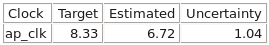
\includegraphics[resolution=100]{fft120_syn_report}\\
\end{center}
\caption{Timing characteristics taken from the C Synthesis Report for MachSuite's Strided FFT, generated by Vivado HLS. Targeting a clock frequency of 120MHz.}
\label{fig:120mhz_syn_report}
\end{figure}
The block diagram shown in Appendix~\ref{app:block_diagram} was synthesized with the peripheral clock (\texttt{FCLK\_CLK0} from the Zynq processor) set to 100MHz and then 120MHz. At each frequency, execution time was recorded for the FFT in software, in hardware using the DMA engine, and in hardware not using the DMA engine. The XTime library from Xilinx was used to time sections of code, as shown in Listing~\ref{lst:time_ex}.

\begin{lstlisting}[caption={XTime example},label={lst:time_ex}]
XTime tStart, tEnd;
XTime_GetTime(&tStart);
// Region of interest goes here
XTime_GetTime(&tEnd);
time = (tEnd - tStart);
xil_printf("Region of interest took %d timer cycles.\n",time);
\end{lstlisting}

The number of timer cycles spent computing each critical section was recorded. Dividing by the timer clock rate yields the time in seconds.
\begin{minipage}{\linewidth}
The following critical sections were selected for timing:
\begin{itemize}
\item Sending inputs to the FFT
\item Computation of the FFT
\item Retrieving results from the FFT\\
\end{itemize}
\end{minipage}

No time was spent sending nor retrieving data in software since it operates on arrays in main memory. The FFT accelerator, on the other hand, requires data to be copied to and from its scratchpad memory. The DMA engine is used to move inputs and outputs between main memory and the FFT's scratchpad memory. When not using the DMA, the Zynq processor must manually copy the data. In all cases, the hardware implementation is synchronous, meaning the Zynq processor initiates each input/output copy one at a time and then must wait while each transfer takes place.

\subsubsection{Results}
\begin{figure}
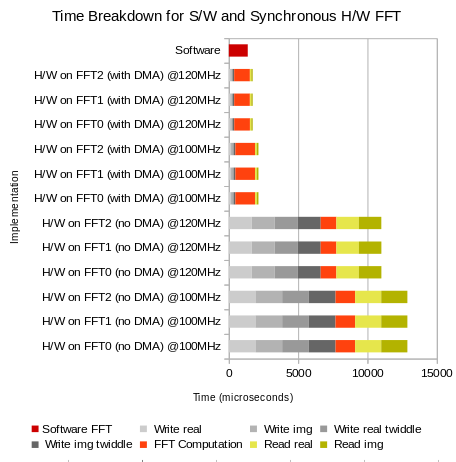
\includegraphics[width=0.47\textwidth]{hw_v_sw_dma_and_no_dma}\\
\caption{Time breakdown of an FFT done in software versus in hardware, showing all implementations (with/without a DMA engine, and with peripherals clocked at 100MHz and 120MHz). Each critical step is highlighted in a different color. Copying of input operands is highlighted in shades of gray, the actual computation in shades of red, and copying back results in shades of yellow.}
\label{fig:hw_sw_all}
\end{figure}

\begin{figure}
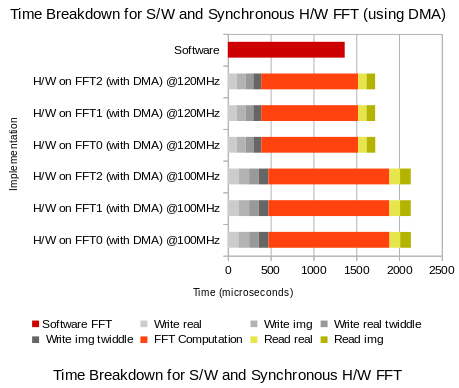
\includegraphics[width=0.47\textwidth]{hw_v_sw_dma}\\
\caption{Close-up view of execution time for the hardware implementations with a DMA engine.}
\label{fig:hw_sw_dma}
\end{figure}

Figures~\ref{fig:hw_sw_all}~and~\ref{fig:hw_sw_dma} show the time spent executing the FFT in software running entirely on the Zynq processor versus each step in hardware under different constraints. The runtime for each of the three FFT accelerators is shown at two different clock rates and with and without a DMA engine.

One will notice that using the DMA drastically speeds up execution. On average, the DMA speeds up all data transfer by approximately 16x as compared to the processor manually copying data. Unsurprisingly, the time spent computing the FFT is unaffected by the use of a DMA engine. Figure~\ref{fig:hw_sw_dma} gives a more close-up view of how the hardware accelerator with DMA compares to software.

When increasing the clock frequency of the FFT accelerator, DMA engine, and AXI interconnect from 100MHz to 120MHz, one can see that every step of the hardware implementation speeds up, whether using the DMA or not. This is because the DMA and the Zynq processor are both constrained in how fast they can transfer data by the speed of the interconnect.

Finally, it is important to note that the software implementation is faster than hardware in all cases in terms of total execution time. However, this includes the time spent copying data to and from the FFT accelerator. In Figure~\ref{fig:hw_sw_dma}, one can see that at 120MHz, the actual computation (shown in red) is completed faster in hardware than in software. The synchronous data transfer which comes before and after computation lengthens execution time such that there is no speedup over the software implementation. Transferring data asynchronously could amortize this overhead by allowing the Zynq processor to do other useful work while data is moved by a DMA.



\section{Project Execution Evaluation}
My original task was to develop an application that uses many accelerators in a way that highlights their varied interactions in a many-accelerator architecture. Along the way, I discovered that designing the underlying architecture itself would take a significant amount of time. Decisions needed to be made about how data would be moved between accelerators, what interface accelerators would need to comply with. To make these decisions and implement them, I needed to learn a number of programs---such as the Xilinx SDK, Vivado, and Vivado HLS---and also research hardware accelerators, accelerator-rich architectures, and general principles for architectural-level design.

Ultimately, I was unable to begin work on the application itself, but I have accomplished an important piece of this project in developing and validating the underlying architecture. To date, I have validated the current architecture design, highlighted areas for improvement and further development, and packaged the architecture so that someone else can easily pick up where I left off.

\newpage

\appendix

\begin{landscape}
\appendixpage
\section{Architecture block diagram}
\label{app:block_diagram}
\begin{figure}[!th]
\centering
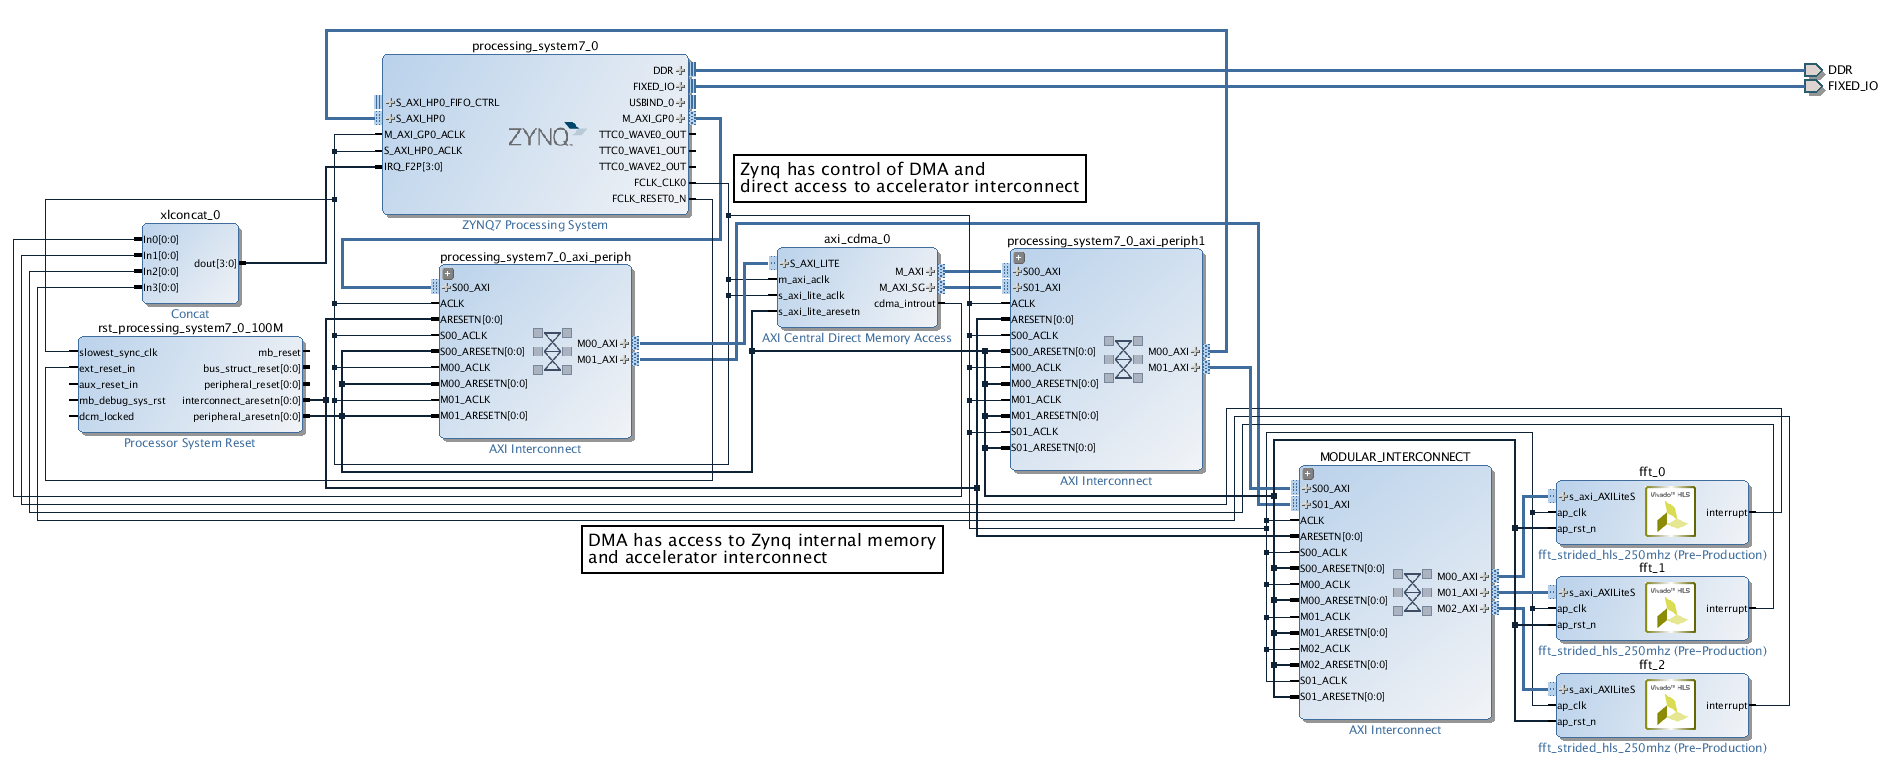
\includegraphics[height=0.50\textheight]{block_diagram}
\caption{The block diagram of the architecture from Vivado.\\Composed of a Zynq processor, AXI Central DMA,\\and three FFT accelerators synthesized by Vivado HLS.}
\end{figure}

\end{landscape}


%%%%%%%%%%%%%  THIS IS WHERE THE BIBLIOGRAPHY GOES %%%%%%%%%

% Change the word "template" below to the name of the .bib file you use
\begin{small}
\bibliographystyle{abbrv} \bibliography{main}
\end{small}

\end{document}

